\section{An Example}

In this section, the proposed algorithm will be applied to the example graph \(G\) (\(n=8\) and \(m=12\)) shown in
Figure \ref{fig:example} in order to determine its chromatic number.  The steps of the algorithm are then traversed
in reverse order to determine a chromatic coloring.

\begin{figure}[h]
  \label{fig:example}
  \begin{center}
    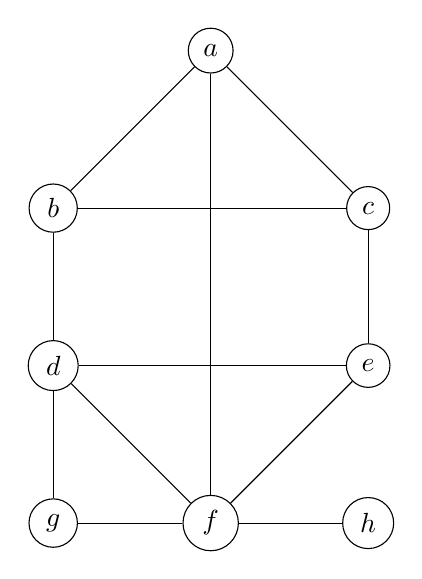
\begin{tikzpicture}
      \node (a) [draw,circle] at (2,6) {\(a\)};
      \node (b) [draw,circle] at (0,4) {\(b\)};
      \node (c) [draw,circle] at (4,4) {\(c\)};
      \node (d) [draw,circle] at (0,2) {\(d\)};
      \node (e) [draw,circle] at (4,2) {\(e\)};
      \node (f) [draw,circle] at (2,0) {\(f\)};
      \node (g) [draw,circle] at (0,0) {\(g\)};
      \node (h) [draw,circle] at (4,0) {\(h\)};
      \draw (a) to (b);
      \draw (a) to (c);
      \draw (a) to (f);
      \draw (b) to (c);
      \draw (b) to (d);
      \draw (c) to (e);
      \draw (d) to (e);
      \draw (d) to (f);
      \draw (d) to (g);
      \draw (e) to (f);
      \draw (f) to (g);
      \draw (f) to (h);
    \end{tikzpicture}
  \end{center}
  \caption{Example Graph}
\end{figure}

The algorithm steps are as follows.  Outer loop steps are marked by ``O\#'' and called subroutine steps are marked by
``I\#.''.  Recursive subroutine calls add a call level: ``I\#--\#.''

\begin{enumerate}
\item (O\ref{step:null}) Since \(n=8>0\), \(G\) is not the null graph, so continue.

\item (O\ref{step:one}) Since \(n=8>1\), \(G\) is not an empty graph, so continue.

\item (O\ref{step:init}) Initialize \(k\) to 2.

\item (O\ref{step:inner}) Call the subroutine with \(G\) and \(k=2\).

\item (I\ref{step:check}) \(n=8\nleq k=2\), so continue.

\item (I\ref{step:dencalc}) Calculate the maximum edge threshold for \(n=8\) and \(k=2\):
  \[a=\frac{n^2(k-1)}{2k}=\frac{8^2(2-1)}{2\cdot2}=\frac{64}{4}=16\]

\item (I\ref{step:density}) Since \(m=12\ngtr16=a\), continue.

\item (I\ref{step:smallcalc}) Since \(\deg(h)=1<2\), set \(X=\set{h}\).

\item (I\ref{step:small}) Since \(X\ne\emptyset\), replace \(G\) with \(G-X\).  The result is shown in Figure
  \ref{fig:removeh}.  Now \(n=7\) and \(m=11\).

  \begin{figure}[h]
    \label{fig:removeh}
    \begin{center}
      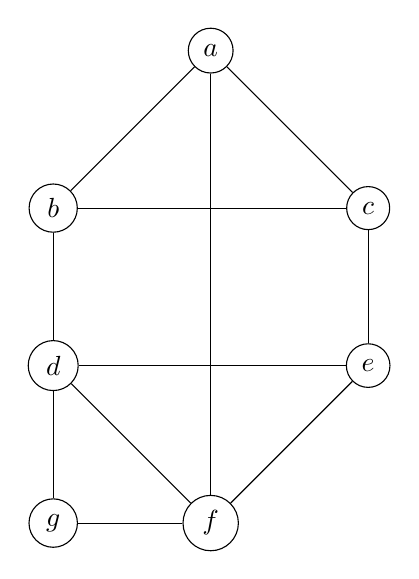
\begin{tikzpicture}
        \node (a) [draw,circle] at (2,6) {\(a\)};
        \node (b) [draw,circle] at (0,4) {\(b\)};
        \node (c) [draw,circle] at (4,4) {\(c\)};
        \node (d) [draw,circle] at (0,2) {\(d\)};
        \node (e) [draw,circle] at (4,2) {\(e\)};
        \node (f) [draw,circle] at (2,0) {\(f\)};
        \node (g) [draw,circle] at (0,0) {\(g\)};
        \draw (a) to (b);
        \draw (a) to (c);
        \draw (a) to (f);
        \draw (b) to (c);
        \draw (b) to (d);
        \draw (c) to (e);
        \draw (d) to (e);
        \draw (d) to (f);
        \draw (d) to (g);
        \draw (e) to (f);
        \draw (f) to (g);
      \end{tikzpicture}
    \end{center}
    \caption{\(G-\set{h}\)}
  \end{figure}

\item (I\ref{step:check}) \(n=7\nleq k=2\), so continue.

\item (I\ref{step:dencalc}) Calculate the maximum edge threshold for \(n=7\) and \(k=2\):
  \[a=\frac{n^2(k-1)}{2k}=\frac{7^2(2-1)}{2\cdot2}=\frac{49}{4}\approx12.3\]

\item (I\ref{step:density}) Since \(m=12\ngtr12.3=a\), continue.

\item (I\ref{step:smallcalc}) Since \(\d(G)=2\ge2=k\), set \(X=\emptyset\).

\item (I\ref{step:small}) Since \(X=\emptyset\), continue.

\item (I\ref{step:subset}) Note that \(N(g)=\set{d,f}\) and \(N(e)=\set{c,d,f}\).  Since \(N(g)\subseteq N(e)\),
  replace \(G\) with \(G-g\).  The result is shown in Figure \ref{fig:removeg}.  Now \(n=6\) and \(m=9\).

  \begin{figure}[h]
    \label{fig:removeg}
    \begin{center}
      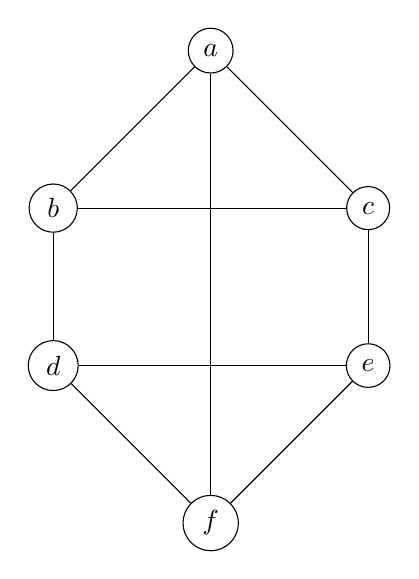
\begin{tikzpicture}
        \node (a) [draw,circle] at (2,6) {\(a\)};
        \node (b) [draw,circle] at (0,4) {\(b\)};
        \node (c) [draw,circle] at (4,4) {\(c\)};
        \node (d) [draw,circle] at (0,2) {\(d\)};
        \node (e) [draw,circle] at (4,2) {\(e\)};
        \node (f) [draw,circle] at (2,0) {\(f\)};
        \draw (a) to (b);
        \draw (a) to (c);
        \draw (a) to (f);
        \draw (b) to (c);
        \draw (b) to (d);
        \draw (c) to (e);
        \draw (d) to (e);
        \draw (d) to (f);
        \draw (e) to (f);
      \end{tikzpicture}
    \end{center}
    \caption{\(G-g\)}
  \end{figure}

\item (I\ref{step:check}) \(n=6\nleq k=2\), so continue.

\item (I\ref{step:dencalc}) Calculate the maximum edge threshold for \(n=6\) and \(k=2\):
  \[a=\frac{n^2(k-1)}{2k}=\frac{6^2(2-1)}{2\cdot2}=\frac{36}{4}=9\]

\item (I\ref{step:density}) Since \(m=9\ngtr9=a\), continue.

\item (I\ref{step:smallcalc}) Since \(\d(G)=2\ge2=k\), set \(X=\emptyset\).

\item (I\ref{step:small}) Since \(X=\emptyset\), continue.

\item (I\ref{step:subset}) Since there is no \(N(u)\subseteq N(v)\), continue.

\item (I\ref{step:select}) Note that due to the symmetry of \(G\) every two vertices share exactly two neighbors:
  \[b=\min_{u,v\in V(G)}\abs{N(u)\cap N(v)]}=2\]

\item (I\ref{step:ubcalc}) Calculate the upper bound for minimum number of common neighbors for \(n=6\) and
  \(k=2\):
  \[c=n-2-\frac{n-2}{k-1}=6-2-\frac{6-2}{2-1}=4-4=0\]

\item (I\ref{step:ubcheck}) Since \(b=2>0=c\), conclude that \(G\) is not \colorable{2}.  Return false and the current
  state of \(G\) to the outer loop.

\item (O\ref{step:call}) Since the called subroutine returned false, \(G\) is not \colorable{2}, so continue.

\item (O\ref{step:newg}) Replace \(G\) with the graph returned by the previous call (Figure \ref{fig:removeg}).

\item (O\ref{step:incr}) Increment \(k\) to 3.

\item (O\ref{step:inner}) Call the subroutine with the new \(G\) and \(k=3\).
  
\item (I\ref{step:check}) \(n=6\nleq k=3\), so continue.

\item (I\ref{step:dencalc}) Calculate the maximum edge threshold for \(n=6\) and \(k=3\):
  \[a=\frac{n^2(k-1)}{2k}=\frac{6^2(3-1)}{2\cdot3}=\frac{72}{6}=12\]

\item (I\ref{step:density}) Since \(m=9\ngtr11=a\), continue.

\item (I\ref{step:smallcalc}) Since \(\d(G)=3\ge3=k\), set \(X=\emptyset\).

\item (I\ref{step:small}) Since \(X=\emptyset\), continue.

\item (I\ref{step:select}) Note that due to the symmetry of \(G\) every two vertices share exactly two neighbors:
  \[b=\min_{u,v\in V(G)}\abs{N(u)\cap N(v)]}=2\]

\item (I\ref{step:ubcalc}) Calculate the upper bound for minimum number of common neighbors for \(n=6\) and
  \(k=3\):
  \[c=n-2-\frac{n-2}{k-1}=6-2-\frac{6-2}{3-1}=4-2=2\]

\item (I\ref{step:ubcheck}) Since \(b=2\ngtr2=c\), continue.

\item (I\ref{step:select2}) Since every two vertices share exactly two neighbors, select any two non-adjacent
  vertices: \(a\) and \(e\).

\item (I\ref{step:call1}) Recursively call the subroutine with \(G\cdot ae\) and \(k=3\).  The result is shown in
  Figure \ref{fig:conae}.  Now \(n=5\) and \(m=7\).

  \begin{figure}[h]
    \label{fig:conae}
    \begin{center}
      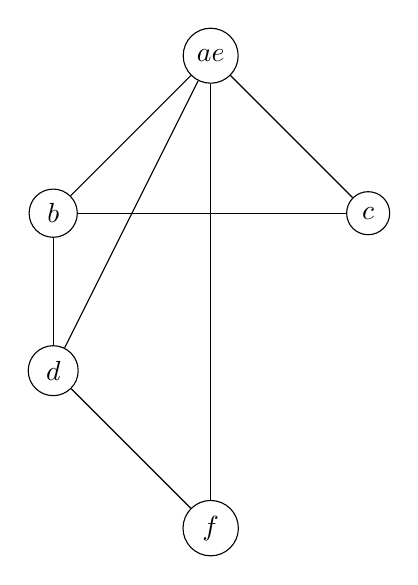
\begin{tikzpicture}
        \node (ae) [draw,circle] at (2,6) {\(ae\)};
        \node (b) [draw,circle] at (0,4) {\(b\)};
        \node (c) [draw,circle] at (4,4) {\(c\)};
        \node (d) [draw,circle] at (0,2) {\(d\)};
        \node (f) [draw,circle] at (2,0) {\(f\)};
        \draw (ae) to (b);
        \draw (ae) to (c);
        \draw (ae) to (f);
        \draw (b) to (c);
        \draw (b) to (d);
        \draw (d) to (ae);
        \draw (d) to (f);
      \end{tikzpicture}
    \end{center}
    \caption{\(G\cdot ae\)}
  \end{figure}

\item (I1-\ref{step:check}) \(n=5\nleq k=3\), so continue.

\item (I1-\ref{step:dencalc}) Calculate the maximum edge threshold for \(n=5\) and \(k=3\):
  \[a=\frac{n^2(k-1)}{2k}=\frac{5^2(3-1)}{2\cdot3}=\frac{50}{6}\approx8.3\]

\item (I1-\ref{step:density}) Since \(m=7\ngtr8.3=a\), continue.

\item (I1-\ref{step:smallcalc}) Since \(\deg(c)=\deg(f)=2<3=k\), set \(X=\set{c,f}\).

\item (I1-\ref{step:small}) Since \(X\ne\emptyset\), replace \(G\) with \(G-X\).  The result is shown in Figure
  \ref{fig:removecf}.  Now \(n=3\) and \(m=3\).

  \begin{figure}[h]
    \label{fig:removecf}
    \begin{center}
      \begin{tikzpicture}
        \node (ae) [draw,circle] at (2,6) {\(ae\)};
        \node (b) [draw,circle] at (0,4) {\(b\)};
        \node (d) [draw,circle] at (0,2) {\(d\)};
        \draw (ae) to (b);
        \draw (b) to (d);
        \draw (d) to (a);
      \end{tikzpicture}
    \end{center}
    \caption{\(G-\set{c,f}\)}
  \end{figure}

\item (I1-\ref{step:check}) \(n=3\le k=3\), so conclude that \(G\) is \colorable{3} and return true.

\item (I\ref{step:call1}) The recursive call returned true, so conclude that \(G\) is \colorable{3} and return true.

\item (O\ref{step:call}) The called subroutine returned true, so conclude that \(G\) is \chromatic{3} and return
  \(\X(G)=3\).

\end{enumerate}

So the algorithm determines that the example \(G\) of Figure \ref{fig:example} is \chromatic{3}.  In order to
determine a \chromatic{3} coloring for \(G\), first construct a set \(C\) of three colors:
\[C=\set{\text{\textcolor{green}{green}},\text{\textcolor{blue}{blue}},\text{\textcolor{red}{red}}}\]
Next, follow the algorithm's modification steps in reverse order and color the corresponding vertices accordingly.
The steps are as follows:

\begin{enumerate}
\item First, color the vertices that are present in the final simplified graph.  Assign each vertex its own color,
  except assign contracted vertices the same color.  This is shown in Figure \ref{fig:cstart}.
  
  \begin{figure}[h]
    \label{fig:cstart}
    \begin{center}
      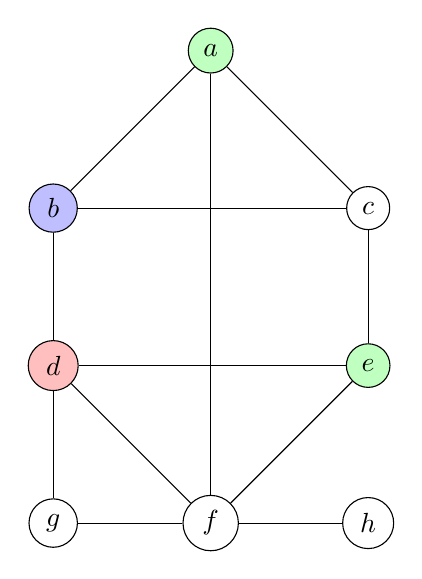
\begin{tikzpicture}
        \colorlet{c1}{green!25!white}
        \colorlet{c2}{blue!25!white}
        \colorlet{c3}{red!25!white}
        \node [fill=c1] (a) [draw,circle] at (2,6) {\(a\)};
        \node [fill=c2] (b) [draw,circle] at (0,4) {\(b\)};
        \node (c) [draw,circle] at (4,4) {\(c\)};
        \node [fill=c3] (d) [draw,circle] at (0,2) {\(d\)};
        \node [fill=c1] (e) [draw,circle] at (4,2) {\(e\)};
        \node (f) [draw,circle] at (2,0) {\(f\)};
        \node (g) [draw,circle] at (0,0) {\(g\)};
        \node (h) [draw,circle] at (4,0) {\(h\)};
        \draw (a) to (b);
        \draw (a) to (c);
        \draw (a) to (f);
        \draw (b) to (c);
        \draw (b) to (d);
        \draw (c) to (e);
        \draw (d) to (e);
        \draw (d) to (f);
        \draw (d) to (g);
        \draw (e) to (f);
        \draw (f) to (g);
        \draw (f) to (h);
      \end{tikzpicture}
    \end{center}
    \caption{Initial Coloring}
  \end{figure}

\item The last modification was the removal of vertices \(c\) and \(f\).  Note that color selection needs to honor
  the vertices already colored.  This is shown in Figure \ref{fig:colorcf}.

  \begin{figure}[h]
    \label{fig:colorcf}
    \begin{center}
      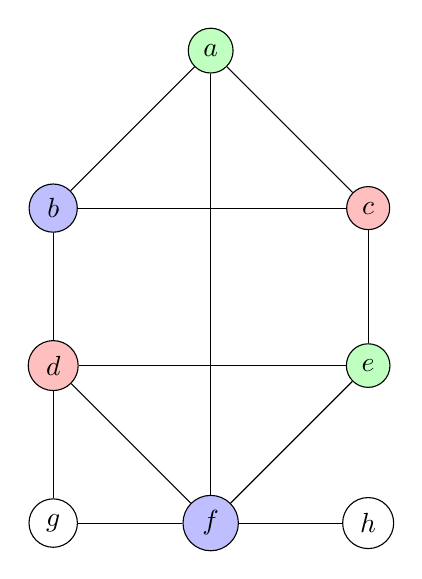
\begin{tikzpicture}
        \colorlet{c1}{green!25!white}
        \colorlet{c2}{blue!25!white}
        \colorlet{c3}{red!25!white}
        \node [fill=c1] (a) [draw,circle] at (2,6) {\(a\)};
        \node [fill=c2] (b) [draw,circle] at (0,4) {\(b\)};
        \node [fill=c3] (c) [draw,circle] at (4,4) {\(c\)};
        \node [fill=c3] (d) [draw,circle] at (0,2) {\(d\)};
        \node [fill=c1] (e) [draw,circle] at (4,2) {\(e\)};
        \node [fill=c2] (f) [draw,circle] at (2,0) {\(f\)};
        \node (g) [draw,circle] at (0,0) {\(g\)};
        \node (h) [draw,circle] at (4,0) {\(h\)};
        \draw (a) to (b);
        \draw (a) to (c);
        \draw (a) to (f);
        \draw (b) to (c);
        \draw (b) to (d);
        \draw (c) to (e);
        \draw (d) to (e);
        \draw (d) to (f);
        \draw (d) to (g);
        \draw (e) to (f);
        \draw (f) to (g);
        \draw (f) to (h);
      \end{tikzpicture}
    \end{center}
    \caption{Coloring \(c\) and \(f\)}
  \end{figure}

\item The contracted vertices have already been colored, so the next simplification to address is the removal of
  \(g\) due to the neighborhood subset test.  Since \(N(g)\subseteq N(e)\), color \(g\) and \(e\) the same color.
  Since \(e\) has already been assign a color, use it for \(g\).  The result is shown in Figure \ref{fig:colorg}.

  \begin{figure}[h]
    \label{fig:colorg}
    \begin{center}
      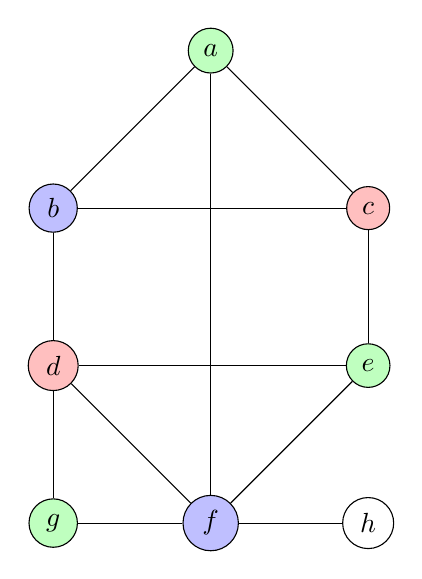
\begin{tikzpicture}
        \colorlet{c1}{green!25!white}
        \colorlet{c2}{blue!25!white}
        \colorlet{c3}{red!25!white}
        \node [fill=c1] (a) [draw,circle] at (2,6) {\(a\)};
        \node [fill=c2] (b) [draw,circle] at (0,4) {\(b\)};
        \node [fill=c3] (c) [draw,circle] at (4,4) {\(c\)};
        \node [fill=c3] (d) [draw,circle] at (0,2) {\(d\)};
        \node [fill=c1] (e) [draw,circle] at (4,2) {\(e\)};
        \node [fill=c2] (f) [draw,circle] at (2,0) {\(f\)};
        \node [fill=c1] (g) [draw,circle] at (0,0) {\(g\)};
        \node (h) [draw,circle] at (4,0) {\(h\)};
        \draw (a) to (b);
        \draw (a) to (c);
        \draw (a) to (f);
        \draw (b) to (c);
        \draw (b) to (d);
        \draw (c) to (e);
        \draw (d) to (e);
        \draw (d) to (f);
        \draw (d) to (g);
        \draw (e) to (f);
        \draw (f) to (g);
        \draw (f) to (h);
      \end{tikzpicture}
    \end{center}
    \caption{Coloring \(g\)}
  \end{figure}

\item Finally, color the first removed vertex \(h\) with any appropriate color.  The final result is shown in
  Figure \ref{fig:cfinal}.

  \begin{figure}[h]
    \label{fig:cfinal}
    \begin{center}
      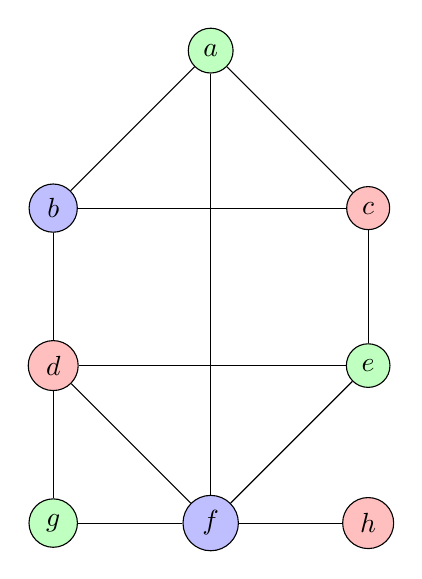
\begin{tikzpicture}
        \colorlet{c1}{green!25!white}
        \colorlet{c2}{blue!25!white}
        \colorlet{c3}{red!25!white}
        \node [fill=c1] (a) [draw,circle] at (2,6) {\(a\)};
        \node [fill=c2] (b) [draw,circle] at (0,4) {\(b\)};
        \node [fill=c3] (c) [draw,circle] at (4,4) {\(c\)};
        \node [fill=c3] (d) [draw,circle] at (0,2) {\(d\)};
        \node [fill=c1] (e) [draw,circle] at (4,2) {\(e\)};
        \node [fill=c2] (f) [draw,circle] at (2,0) {\(f\)};
        \node [fill=c1] (g) [draw,circle] at (0,0) {\(g\)};
        \node [fill=c3] (h) [draw,circle] at (4,0) {\(h\)};
        \draw (a) to (b);
        \draw (a) to (c);
        \draw (a) to (f);
        \draw (b) to (c);
        \draw (b) to (d);
        \draw (c) to (e);
        \draw (d) to (e);
        \draw (d) to (f);
        \draw (d) to (g);
        \draw (e) to (f);
        \draw (f) to (g);
        \draw (f) to (h);
      \end{tikzpicture}
    \end{center}
    \caption{Final Chromatic Coloring}
  \end{figure}

\end{enumerate}

At first glance, one might wonder what advantage this method of coloring has over greedy coloring.  The difference
is that greedy coloring only has knowledge about what has already been colored, whereas this method uses
assumptions that are made during the simplifications and recursive calls on the entire graph.  Thus, the greedy
algorithm is heuristic, but this method selects a particular workable coloring path through the modified Zykov
tree.  In this way, this method is not so much different from the exhaustive algorithm.
